\documentclass[aspectratio=169,11pt]{beamer}

\usepackage[utf8]{inputenc}
\usepackage[T1]{fontenc}
\usepackage[french]{babel}
\usepackage{booktabs}
\usepackage{graphicx}
\usetheme[progressbar=frametitle,numbering=fraction]{metropolis}

\definecolor{accent}{HTML}{004488}
\definecolor{warm}{HTML}{B84A00}
\definecolor{ink}{HTML}{14202B}
\setbeamercolor{frametitle}{bg=ink,fg=white}
\setbeamercolor{progress bar}{fg=accent,bg=accent!20}
\setbeamercolor{alerted text}{fg=warm}
\setbeamercolor{normal text}{fg=ink,bg=white}
\setbeamercolor{example text}{fg=accent}
\graphicspath{{figures/}}
\newcommand{\teff}{$T_{\mathrm{eff}}$}
\newcommand{\bignum}[1]{{\usebeamercolor[fg]{example text}\Huge\bfseries #1}}

\title{Classer les étoiles par leur seul spectre}
\subtitle{APOGEE DR17, version complète : catalogue allStar et 100\,000 étoiles}
\author{Félix Dubé \and Imran Akki \and Charles-Antoine Fournier \and Youssef Lahrichi \and Bastien Posez}
\institute{GIF-4101 / GIF-7005 / GIF-7015 \quad Université Laval}
\date{Décembre 2026}

\begin{document}

\maketitle

\begin{frame}{La question}
\begin{center}
\Large Un algorithme retrouve-t-il naines, sous-géantes, géantes rouges et red clump à partir du \alert{spectre seul} ?
\end{center}
\vspace{1em}
\begin{itemize}
  \item Garcia-Dias et al.\ (2018) : K-means sur APOGEE sépare ces classes, mais dépend de l'initialisation.
  \item Version 1 : catalogue allégé, 30\,781 étoiles.
  \item Version complète : catalogue \texttt{allStar} (4\,Go), \alert{99\,773 étoiles}, étiquettes plus riches.
\end{itemize}
\end{frame}

\begin{frame}{Ce que le catalogue complet ajoute}
\begin{columns}[T]
\column{0.55\textwidth}
\begin{itemize}
  \item \textbf{FPARAM} : l'ajustement brut, publié même pour les étoiles rejetées. 2\,815 mauvais spectres gagnent une étiquette.
  \item \textbf{[Mg/Fe] et [Fe/H]} : disque mince et disque épais par la ligne de Weinberg et al.\ (2019).
  \item \textbf{Distance Gaia} : le bulbe se définit par la distance au centre galactique ($< 3$\,kpc).
\end{itemize}
\column{0.4\textwidth}
\bignum{12}\\ étoiles sans classe\\(802 en version 1)\\[0.8em]
\alert{FPARAM n'est pas calibré} : \teff{} plus bas de 75\,K en médiane.
\end{columns}
\end{frame}

\begin{frame}{Les données}
\begin{columns}[T]
\column{0.32\textwidth}
\bignum{66\,372}\\ bons spectres\\[0.8em]
{\usebeamercolor[fg]{alerted text}\Huge\bfseries 33\,401}\\ mauvais spectres\\[0.8em]
\small 69\,\% des mauvais ont un SNR $\geq 70$ : un drapeau les écarte, pas le bruit.
\column{0.66\textwidth}
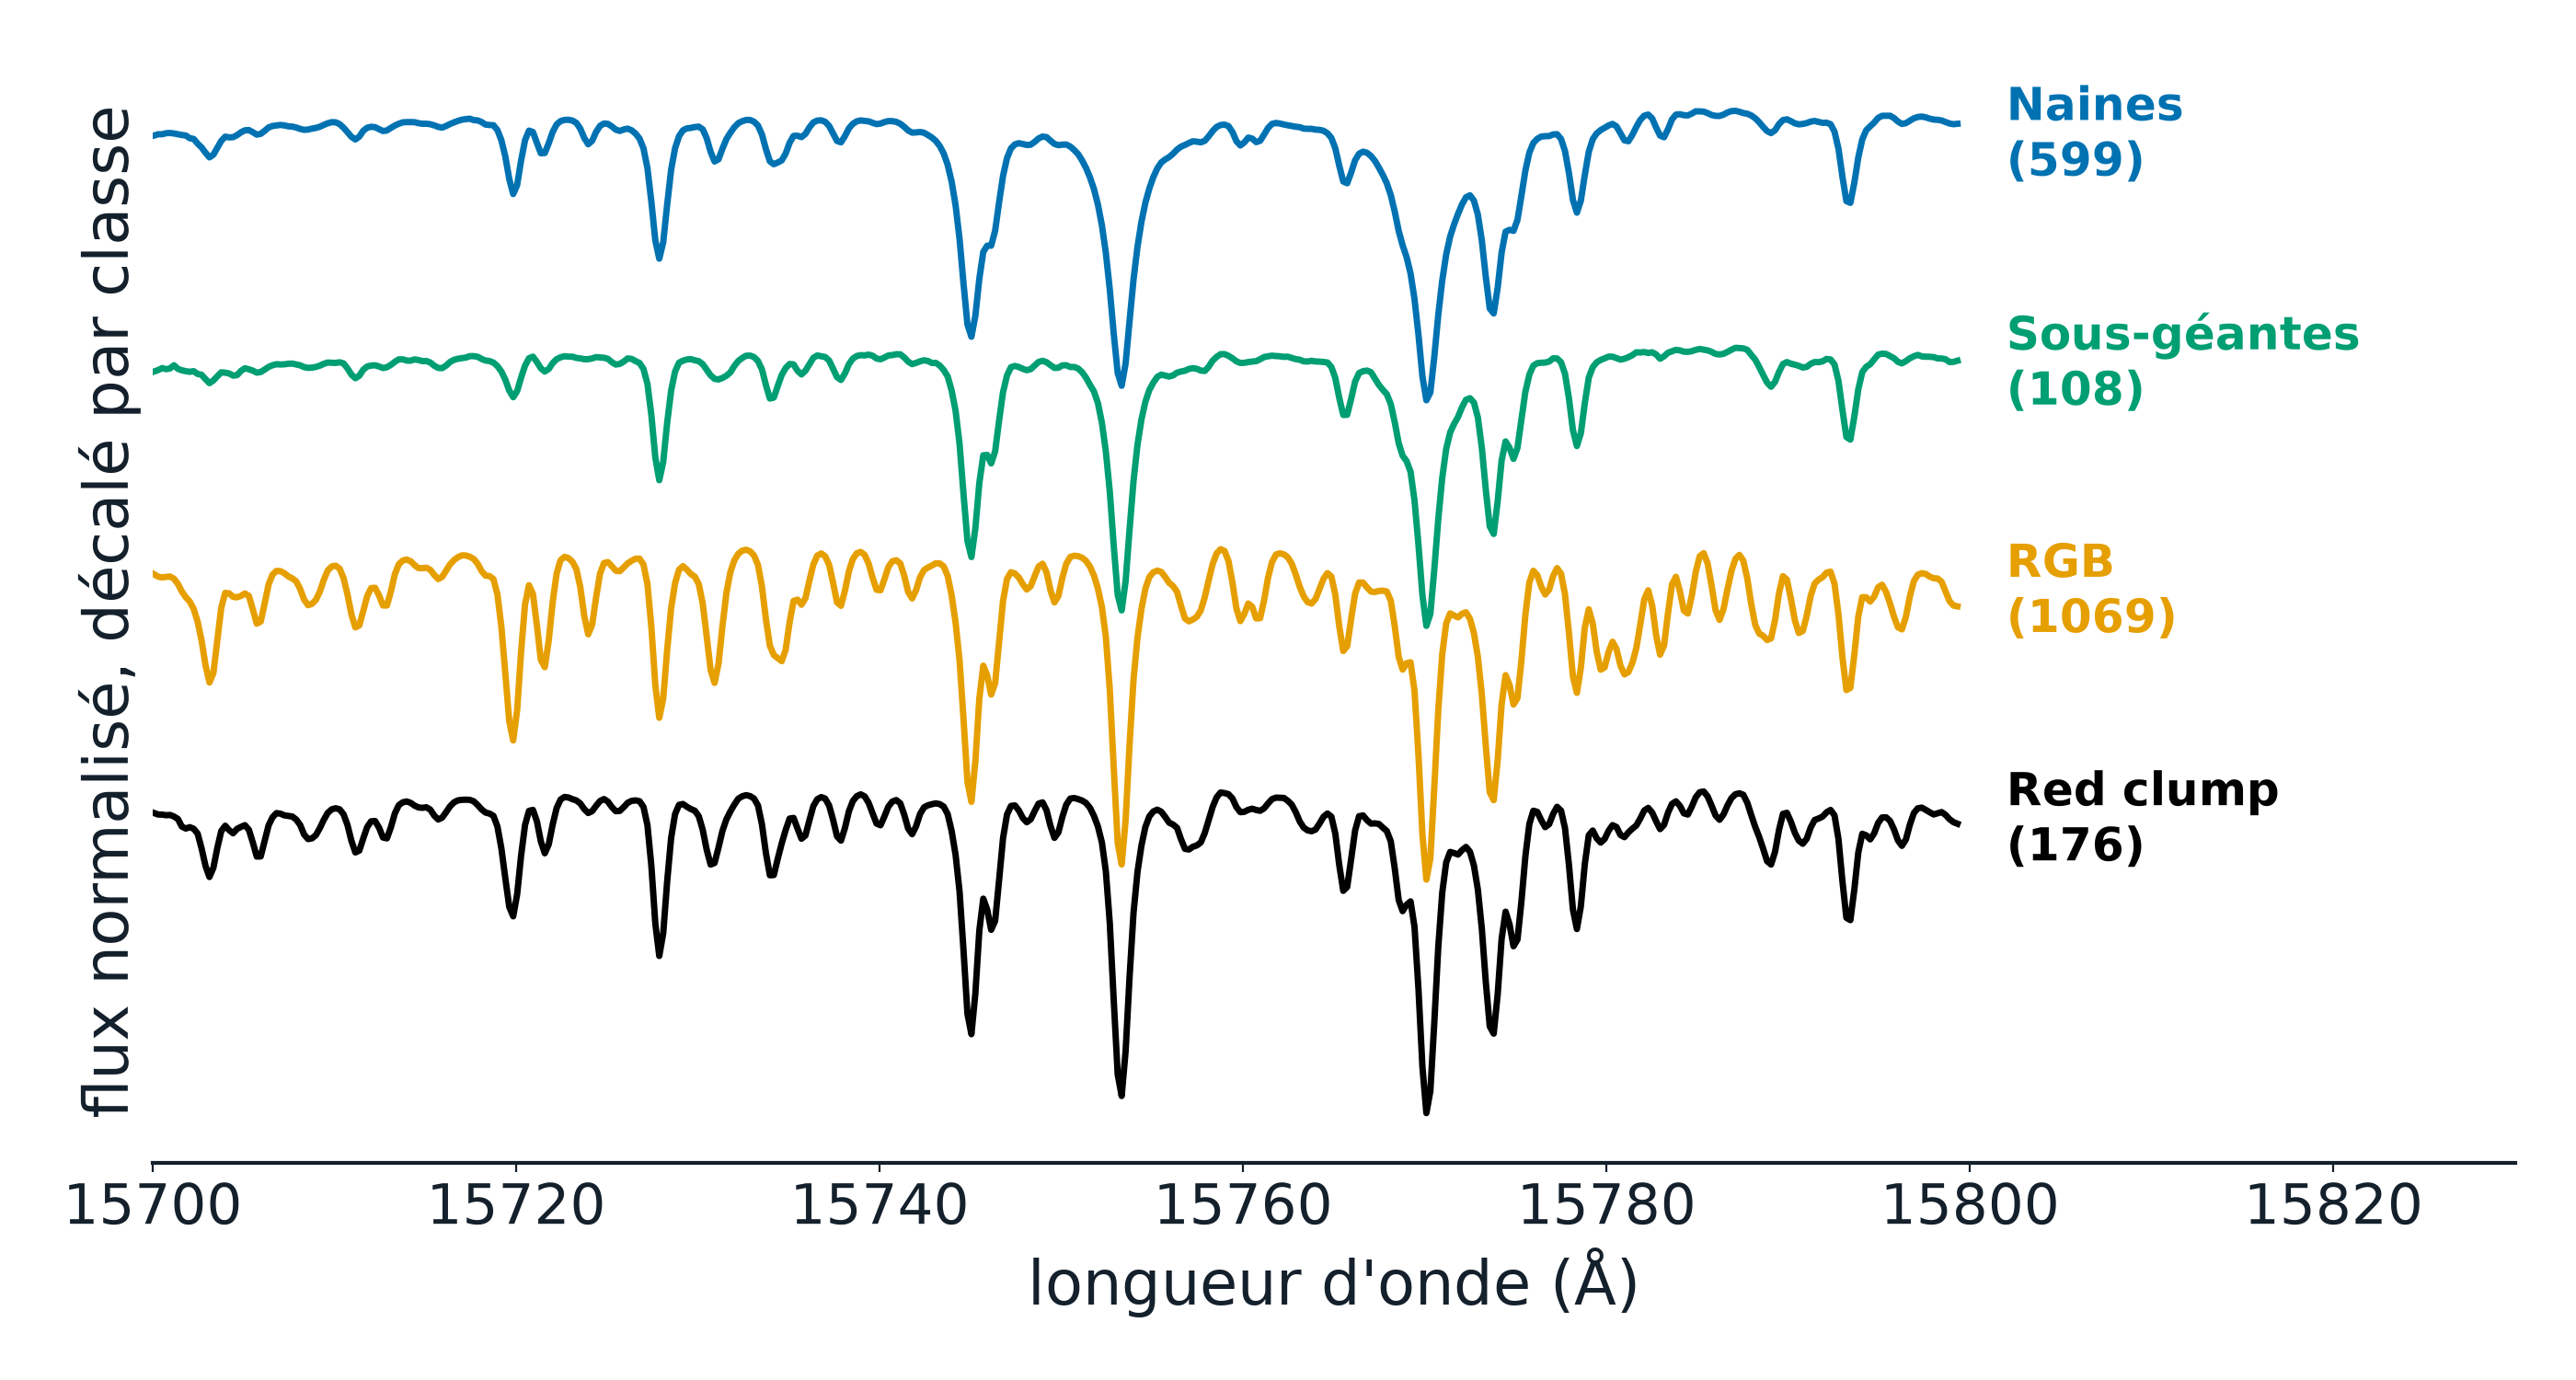
\includegraphics[width=\linewidth]{mean_spectra_zoom.png}\\
\small Spectre moyen par classe sur 100\,Å.
\end{columns}
\end{frame}

\begin{frame}{Méthode}
\begin{columns}[T]
\column{0.48\textwidth}
\textbf{Non supervisé}
\begin{enumerate}
  \item PCA (10 composantes) ou autoencodeur
  \item K-means, GMM, HDBSCAN
  \item $k$ par silhouette et stabilité
  \item Validation : ARI, NMI, amas ouverts
\end{enumerate}
\column{0.48\textwidth}
\textbf{Supervisé}
\begin{enumerate}
  \item Forêt aléatoire sur PCA
  \item CNN 1-D, 150\,000 paramètres
  \item 4 classes, ou \teff, $\log g$, [M/H]
\end{enumerate}
\vspace{0.5em}
Chaque modèle s'entraîne sur les bons spectres, puis sur tous.
\end{columns}
\end{frame}

\begin{frame}{Sans étiquettes, naines et géantes se séparent}
\centering
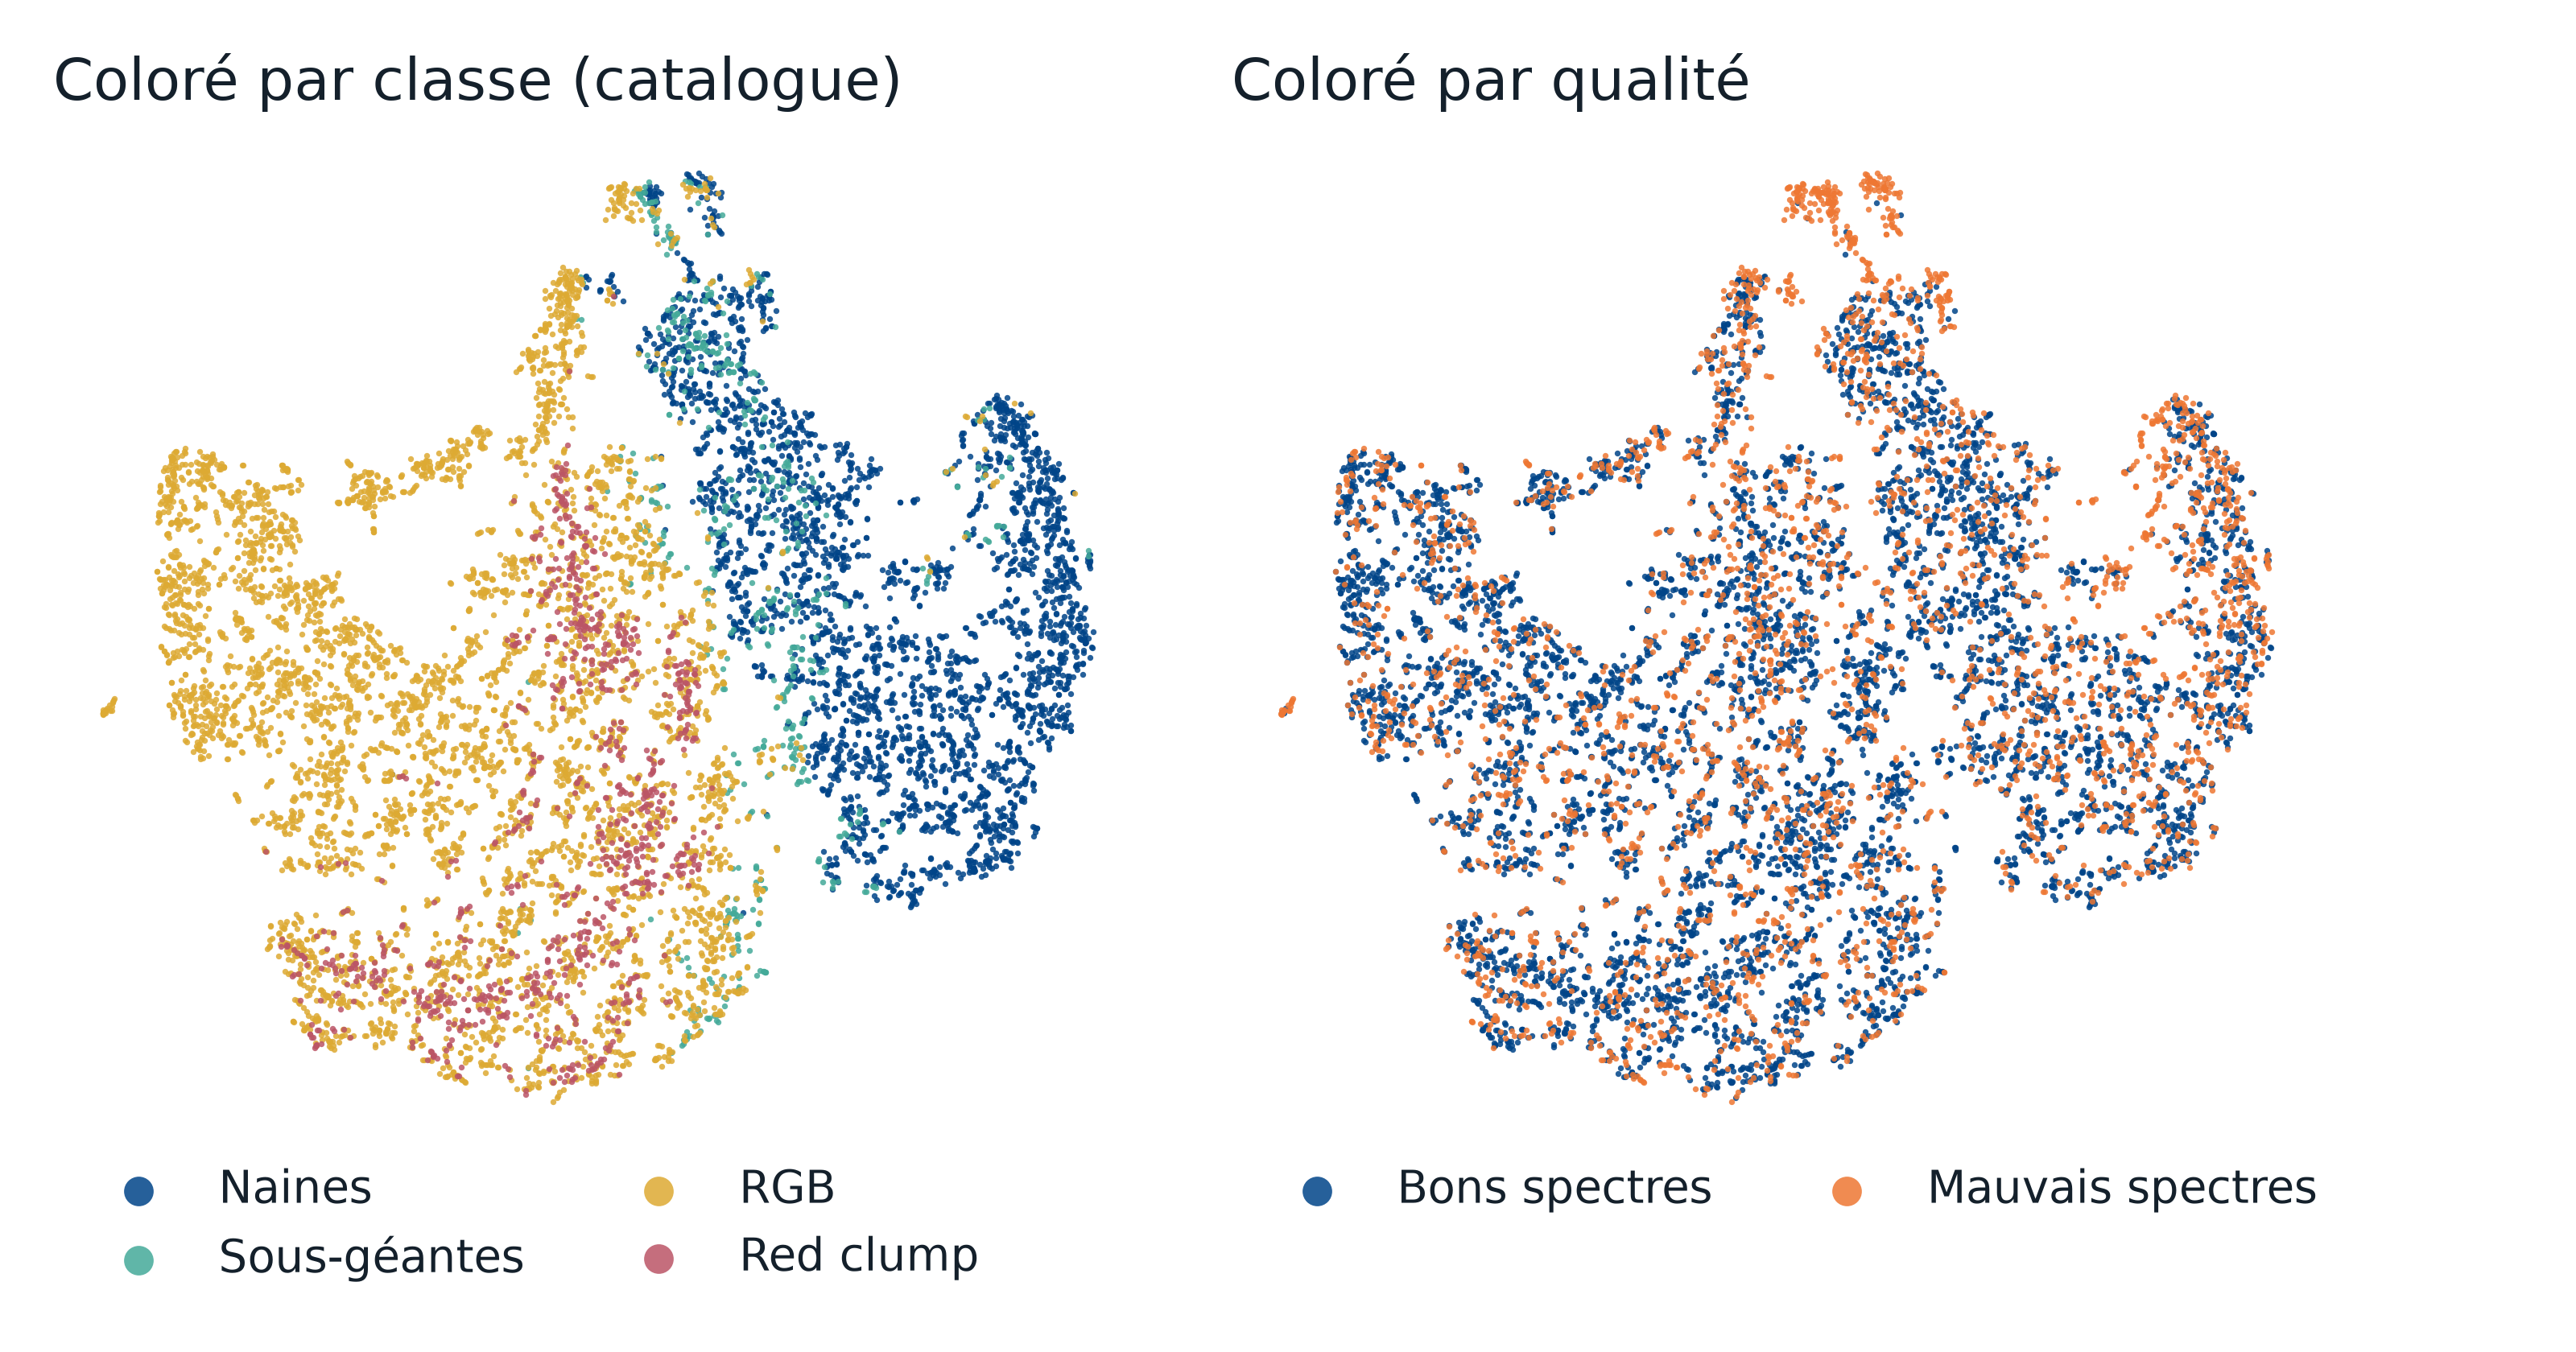
\includegraphics[width=0.78\linewidth]{tsne.png}\\
\small t-SNE de 10\,000 étoiles. Le red clump reste mêlé à la RGB.
\end{frame}

\begin{frame}{Le GMM retrouve les classes évolutives}
\begin{columns}[c]
\column{0.5\textwidth}
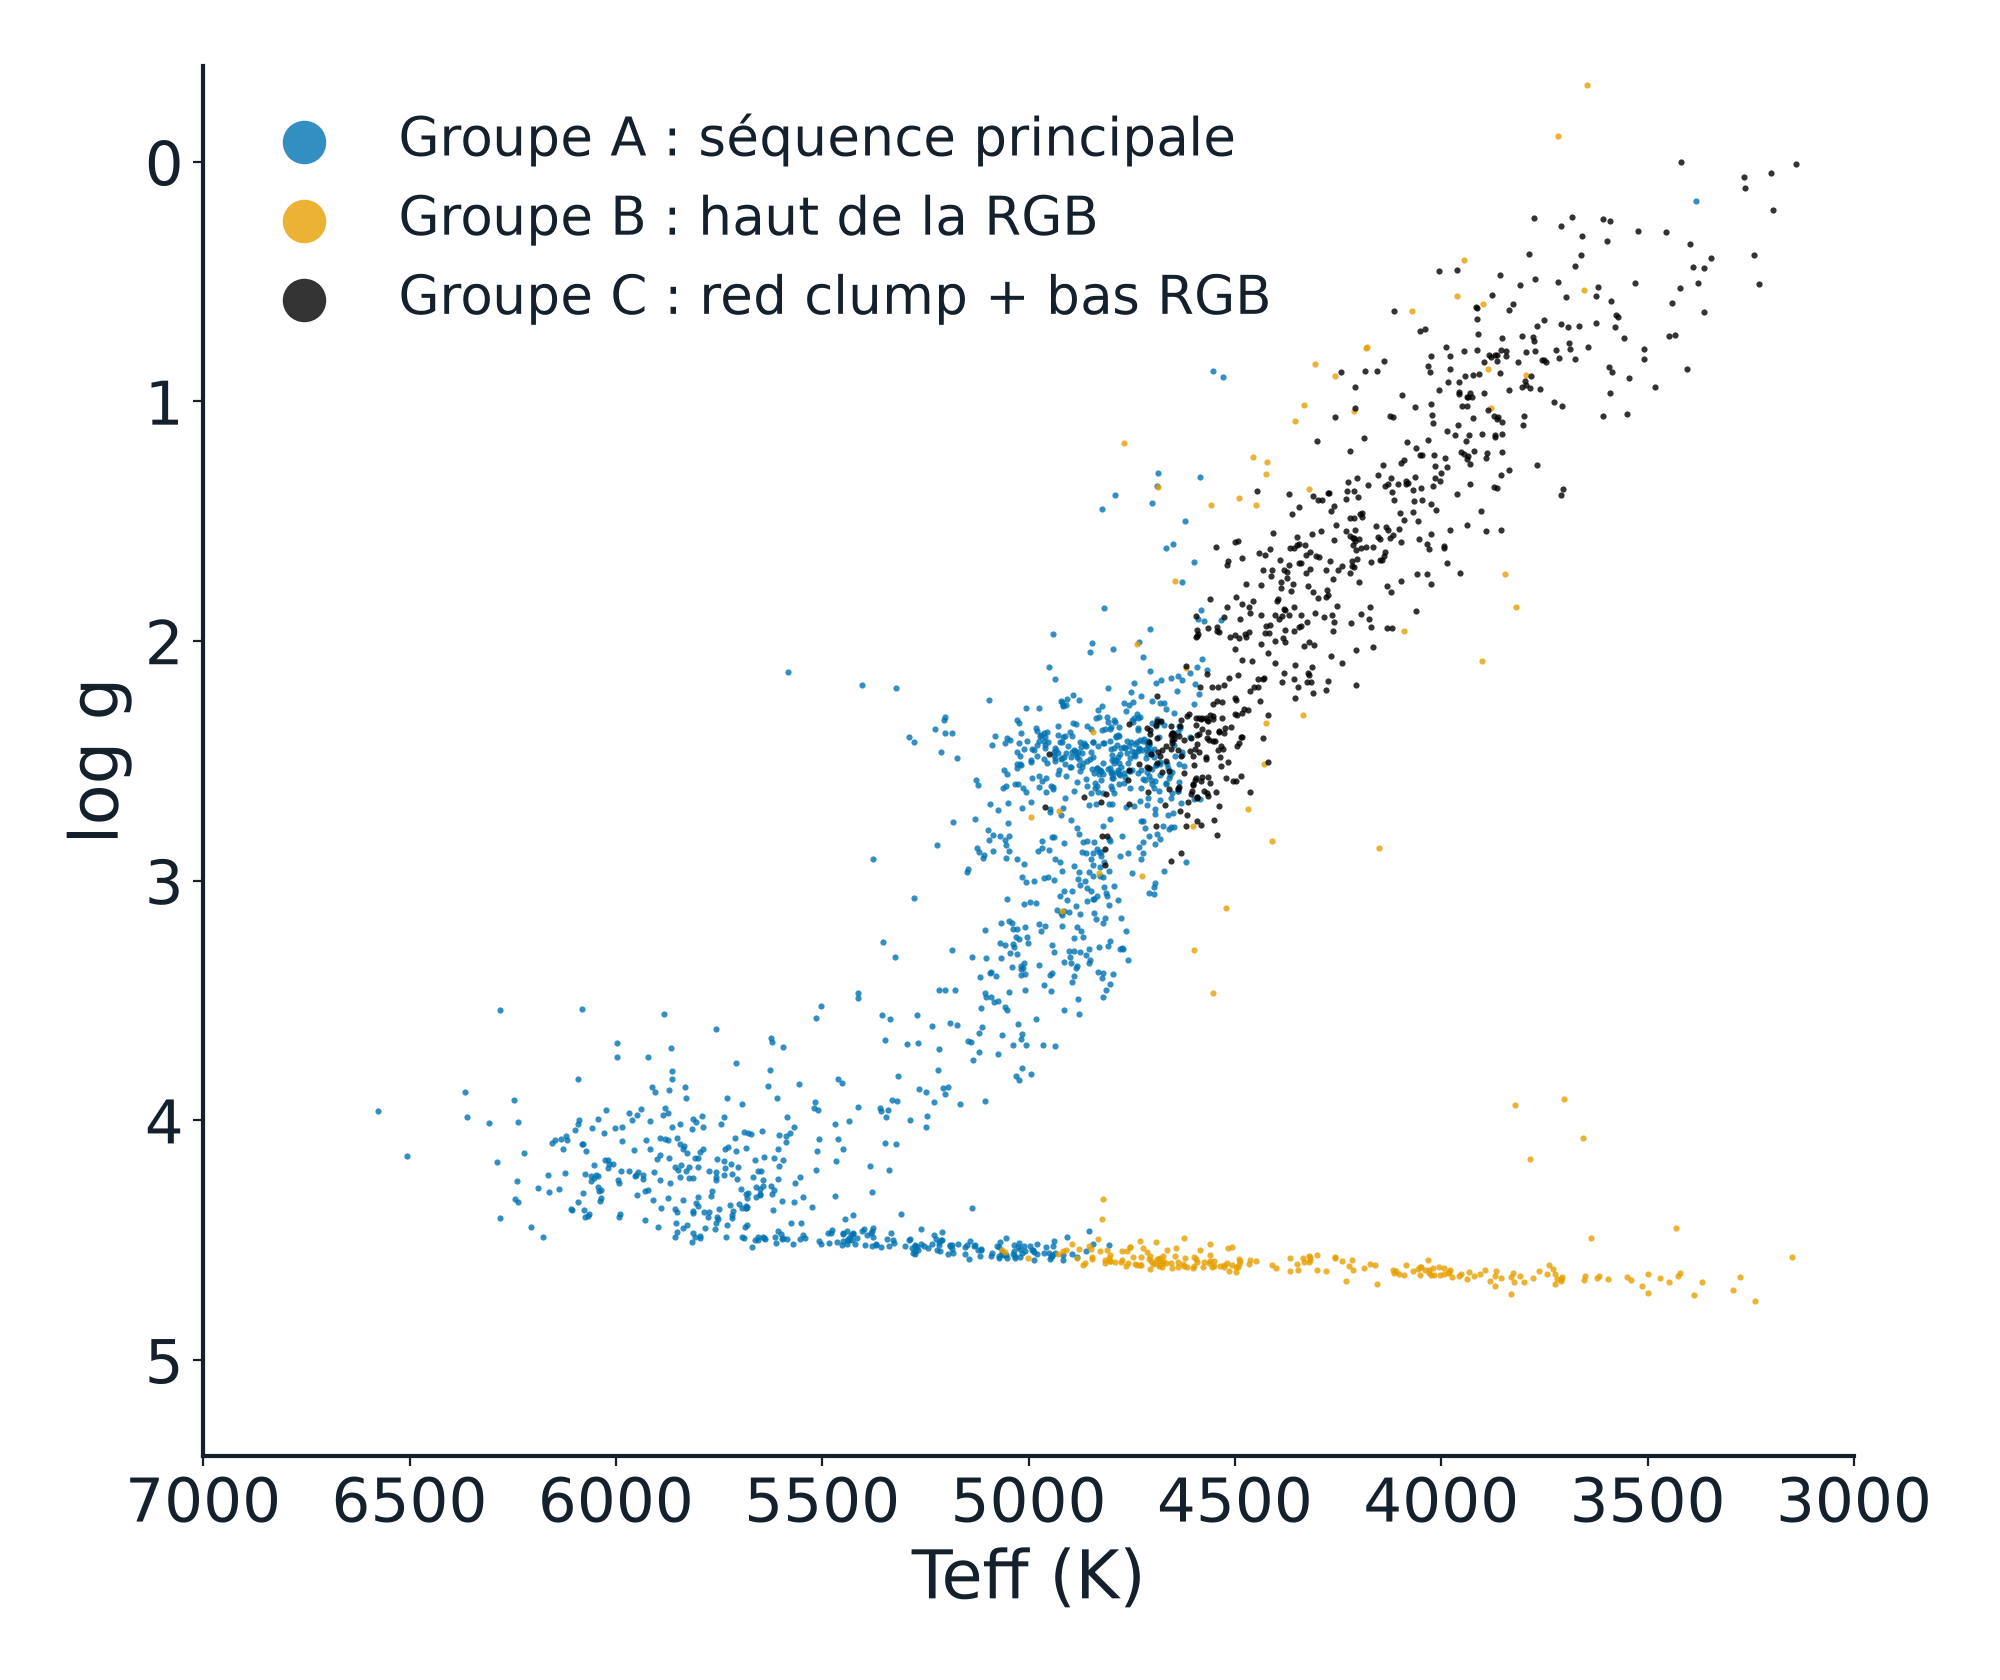
\includegraphics[width=\linewidth]{kiel_gmm.png}
\column{0.46\textwidth}
\bignum{19\,800 / 19\,804}\\ naines dans le groupe A\\[0.8em]
\bignum{97\,\%}\\ du red clump dans le groupe C\\[0.8em]
ARI 0,42 à $k = 3$, \textbf{0,44 à $k = 4$}\\
Populations : ARI $\leq 0{,}13$
\end{columns}
\end{frame}

\begin{frame}{Supervisé : le CNN lit les raies}
\centering
\begin{tabular}{llrrrr}
\toprule
\texttt{test\_good} & Entraînement & Macro F1 & \teff{} (K) & $\log g$ (dex) & [M/H] (dex) \\
\midrule
Forêt & bons & 0,75 & 30,0 & 0,131 & 0,047 \\
Forêt & tous & 0,78 & \textbf{28,1} & 0,108 & 0,042 \\
CNN & bons & 0,83 & 32,9 & \textbf{0,069} & \textbf{0,025} \\
CNN & tous & \textbf{0,86} & 53,7 & 0,102 & 0,030 \\
\bottomrule
\end{tabular}\\[1.2em]
\raggedright
\begin{itemize}
  \item Le CNN divise par deux l'erreur sur $\log g$ et [M/H].
  \item Red clump : 60\,\% de rappel, 40\,\% classé RGB.
\end{itemize}
\end{frame}

\begin{frame}{Mauvais spectres : oui pour classer, non pour mesurer}
\begin{columns}[c]
\column{0.5\textwidth}
\textbf{Classification} : gain dans toutes les tranches de SNR.\\[0.5em]
\small
\begin{tabular}{lrr}
\toprule
SNR & F1 bons & F1 tous \\
\midrule
5 à 30 & 0,42 & \textbf{0,52} \\
30 à 70 & 0,71 & \textbf{0,76} \\
70 à 150 & 0,78 & \textbf{0,81} \\
$> 150$ & 0,84 & \textbf{0,87} \\
\bottomrule
\end{tabular}
\column{0.46\textwidth}
\textbf{Régression} : sur les bons spectres, \teff{} passe de 33 à \alert{54\,K}.\\[0.8em]
Cause : les étiquettes des mauvais spectres. Sur les 417 étoiles FPARAM, l'erreur atteint \alert{874\,K}.
\end{columns}
\end{frame}

\begin{frame}{30\,000 contre 100\,000 étoiles}
\centering
\begin{tabular}{lrr}
\toprule
Mesure (\texttt{test\_good}) & 30\,781 & 99\,773 \\
\midrule
Macro F1, CNN & 0,818 & 0,834 \\
Macro F1, forêt & 0,696 & 0,751 \\
Erreur \teff{}, CNN (K) & 44,6 & 32,9 \\
Erreur $\log g$, CNN (dex) & 0,083 & 0,069 \\
ARI, GMM, $k = 4$ & 0,09 & 0,44 \\
\bottomrule
\end{tabular}\\[1em]
\raggedright
Plus de données aide le supervisé. La limite red clump / RGB demeure.
\end{frame}

\begin{frame}{Temps de calcul}
\centering
\begin{tabular}{lr}
\toprule
Étape & Temps \\
\midrule
Téléchargement des 99\,785 spectres & 87 min (une fois) \\
CNN, 30 époques & 4 à 5,5 min \\
Forêt aléatoire & 0,5 à 2 min \\
Clustering & 1 à 2,5 min \\
\midrule
\textbf{Expérience complète} & \textbf{40 min} \\
\bottomrule
\end{tabular}\\[1em]
RTX 3060 portable (6 Go), 16 threads, 15 Go de RAM.
\end{frame}

\begin{frame}{Limites et suite}
\begin{columns}[T]
\column{0.48\textwidth}
\textbf{Limites}
\begin{itemize}
  \item Étiquettes ASPCAP.
  \item Une seule graine par modèle.
  \item Distances du bulbe incertaines.
\end{itemize}
\column{0.48\textwidth}
\textbf{Suite}
\begin{enumerate}
  \item Régression sur tous les spectres, étiquettes ASPCAP seulement.
  \item 5 graines par modèle.
  \item Red clump / RGB par astérosismologie.
\end{enumerate}
\end{columns}
\end{frame}

\begin{frame}{À retenir}
\begin{enumerate}
  \setlength{\itemsep}{1em}
  \item \textbf{Le spectre seul sépare naines et géantes, sans étiquettes} (GMM, ARI 0,44).
  \item \textbf{Avec étiquettes, le CNN atteint un macro F1 de 0,86.}
  \item \textbf{Les mauvais spectres aident à classer, mais leurs étiquettes bruitées nuisent à la régression.}
\end{enumerate}
\vspace{1.5em}
\small Code : \url{github.com/imranakki/apogee-stars-full}
\end{frame}

\begin{frame}[standout]
Merci. Questions ?
\end{frame}

\end{document}
